\chapter{Project Management}

Project management is an essential part of any project to ensure it runs smoothly and within schedule. So to help manage this project SCRUM was chosen, an iterative process divided into sections with a timespan 1 to 2 weeks called sprints.
The choice was made based on all team members previously had been to a SCRUM-course and had prior experience with it the use of SCRUM.

The process/pipeline for a feature to be implemented must go through the following steps:

\begin{enumerate}
	\item New features
	\item Product backlog
	\item Sprint backlog
	\item In progress
	\item Quality Assurance
	\item Closed/Done
\end{enumerate}

Every feature starts out in the 'New features' section, where each team-member adds the features they would like to see in the finished product if not already listed.

Then at the next meeting features in the 'New features' will be discussed whether to be implemented or not. If the choice is to implement it, it will be put into the 'Product backlog'.

Then at the start of a new sprint, it's discussed which features in 'Product backlog' should be made within the sprint, and those are moved to 'Sprint backlog' and a team-member is assigned as the responsible.

When the feature is stared it's moved into 'In progress'. Then when the developer considers it done it's moved into 'Quality Assurance' where another team member than the developer must quality assure the developed feature and then move it into 'Closed/Done' or 'In progress'.

To help manage the different steps ZenHub was used, it's a planning board with burndown charts and more integrated with Github, the version control service used to keep track of all files. An example of the board can be seen in figure \ref{fig:Zenhub1} and \vref{fig:Zenhub2}

\begin{figure}
	\centering
	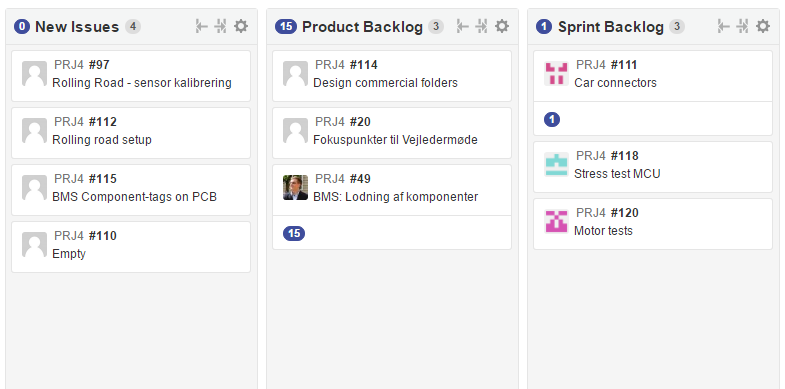
\includegraphics[width=0.7\linewidth]{SubPages/Images/Zenhub1}
	\caption{The 'New issues', 'Product backlog' and 'Sprint backlog' steps}
	\label{fig:Zenhub1}
\end{figure}

\begin{figure}
	\centering
	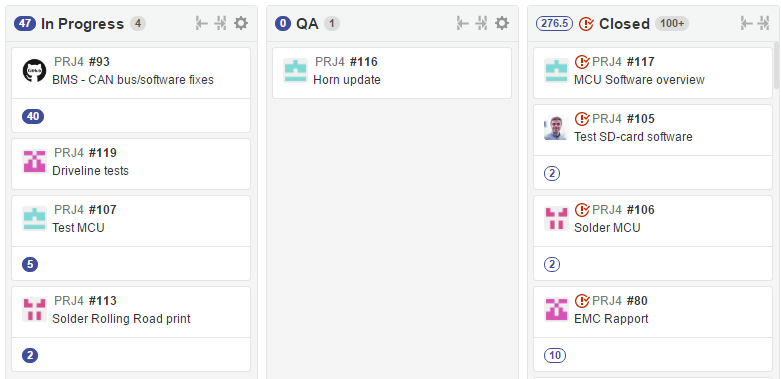
\includegraphics[width=0.7\linewidth]{SubPages/Images/Zenhub2}
	\caption{The 'In progress', 'QA' and 'Closed' steps}
	\label{fig:Zenhub2}
\end{figure}
